\section{Deep Learning}
Deep neural networks (DNNs) have revolutionized the field of NLP along with many others. NLP has seen three main architectures emerge over time: fully connected neural networks (FCNN), recurrent neural networks (RNNs), and Transformers.

\subsection{Fully Connected Neural Networks}
FCNNs are the simplest form of neural networks and are characterized by their feedforward structure, where the input is mapped to one or more output nodes, and with an adjustable number of hidden layers in between.
Each node is connected to every other node in the previous and following layer, via a linear transformation (i.e. a matrix multiplication) followed by a non-linear activation function (e.g. a sigmoid).
The addition of a non-linear activation function allows for the capture of non-linear relationships between the input and output, without it the transformation could be rewritten as just a single matrix multiplication.
The key advantage of DNNs is their ability to automatically learn complex representations of the input data using multiple hidden layers, allowing for the capture of high-level features that could not be easily hand-engineered.

\begin{figure}[h]
    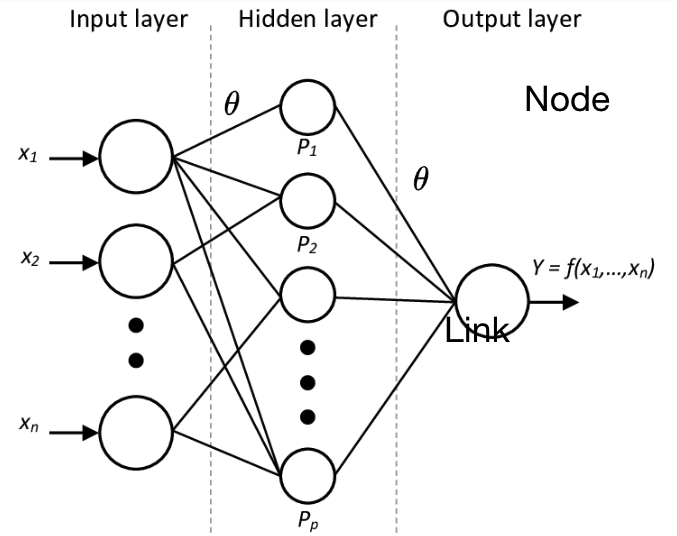
\includegraphics[width=\linewidth]{chapters/NLP/figures/model_architecture.png}
    \caption{Deep neural network architecture}
    \label{fig:model_architecture}
\end{figure}

While glossing over some details, training any type of DNN can summarized in the following steps:
\begin{itemize}
    \item Given data pairs $(x_i, y_i)$, where $x_i$ is an input sample, and $y_i$ is the desired output
    \item Determine a function $f$, such that $f(\theta, x_i) = \hat{y}_i \approx y_i$, where $\theta$ are model parameters and $f$ is the model architecture
    \item Define a loss function $L(\theta) = \sum_i L(\hat{y}_i, y_i)$ that measures how close the model's output is to the desired output
    \item Optimize $\theta$ to minimize $L(\theta)$
\end{itemize}
\begin{figure}[h]
    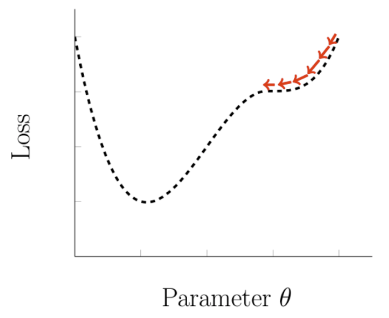
\includegraphics[width=\linewidth]{chapters/NLP/figures/loss.png}
    \caption{Minimizing the loss function}
    \label{fig:loss}
\end{figure}
Here the loss function can take on many forms, depending on the training task, we summarize some of the most common ones in Table \ref{table:losses}.
\begin{table}
    \centering
    \renewcommand{\arraystretch}{1.3}
    \begin{tabular}{|c| c| c|}
    Loss Name & Function & Use \\[0.5ex] \hline
    Mean Squared Error & $\begin{array} {lcl} \frac{1}{N} \sum_{i=1}^N|\hat{y}_i - y_i|^2\end{array}$  & regression \\ [0.5ex]
    Binary Cross Entropy & $\begin{array} {r@{}l@{}} -\frac{1}{N} \sum_{i=1}^N (y_i \cdot log(\hat{y}_i) + (1 - y_i) \cdot log(1-\hat{y}_i)) \end{array}$ & binary classification \\ [0.5ex]
    Cross Entropy & $\begin{array} {r@{}l@{}} -\frac{1}{N} \sum_{i=1}^N y_i \cdot log(\hat{y}_i) \end{array}$ & multiclass classification \\ [0.5ex]
    \end{tabular}
    \caption{Loss functions}
    \label{table:losses}
\end{table}
Training is then formulated as the task of finding the parameter configuration that minimizes the loss function.
We visualize the loss function of just a single parameter in Fig. \ref{fig:loss}.
In order to move towards the global minimum we need to update the parameters in the direction of the steepest descent, which can be calculated by taking the derivative of the loss function with respect to the parameter.
Parameters in the last layer are then updated according to the following rule until convergence
\begin{equation}
    \label{eq:optimization}
    \theta \rightarrow \theta - \alpha \frac{\partial L}{\partial \theta}
\end{equation}
where $\alpha$ is called the \textit{learning rate} and determines the step size, the partial derivative of the loss function with respect to the parameters is called the \textit{gradient}.
Consequently the algorithm is called \textit{Gradient Descent} and is the workhorse of all modern deep learning.
The algorithm trivially extends to the case of multiple parameters in the last layer.
A similar rule applies to parameters in the hidden layers.
Once the gradients of the subsequent layer have been computed we can apply the chain rule from calculus to compute the gradients of the parameters in the current layer -- this is called \textit{Backpropagation}\footnote{Backpropagation}.
% \footnote{https://en.wikipedia.org/wiki/Backpropagation}.

Simple FCNNs have several limitations in NLP.
For example, it is difficult to capture the sequential structure of text data, and they do not scale well to large vocabularies.
Remember, that in order to represent a word in a FCNN, we need to have a one-hot vector of size $|V|$.
To represent a sentence of length $n$, we need to have $n$ vectors of size $|V|$, which is a lot of parameters.

\subsection{Recurrent Neural Networks}
To overcome this, RNNs were introduced.
\begin{figure}[h]
    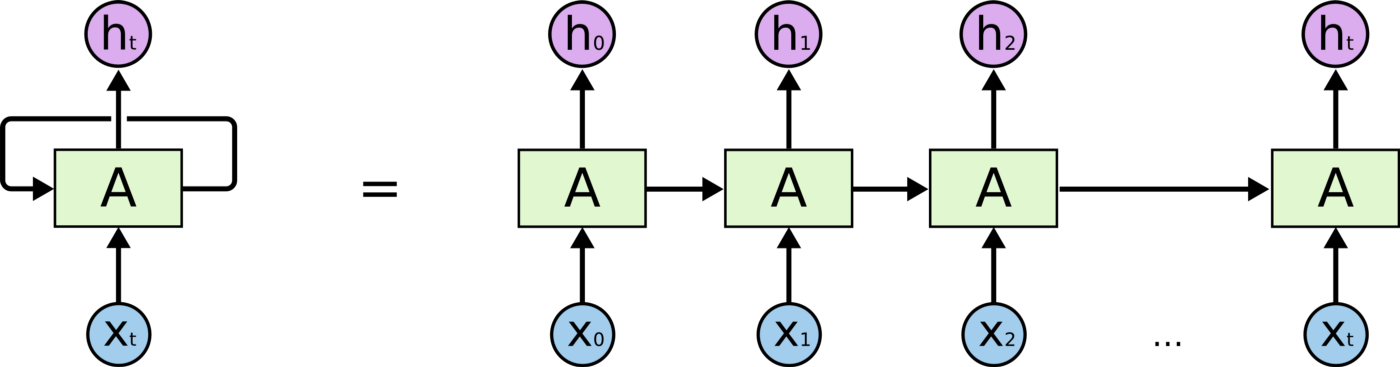
\includegraphics[width=\linewidth]{chapters/NLP/figures/rnn.png}
    \caption{Recurrent Neural Networks capture the sequential nature of text data by using loops in their structure that allow information to flow both forward and backward through the network.}
    \label{fig:rnn}
\end{figure}
RNNs are a type of neural network that have loops in their structure, allowing information to flow both forward and backward through the network (see Fig. \ref{fig:rnn}).
The idea is that we can use the output of the previous step as input to the current step, and the output of the current step as input to the next step and so on.
To encode the meaning of a sentence or paragraph, the model reads the tokens one by one, updating the representation in the hidden state, which can then be used for subsequent predictions.
This allows us to reuse a large part of the parameters, which is crucial for efficient training.
It also means that this architecture is suitable to varying length inputs, as we can stop reading the input once we reach the end of the sentence, which is in contrast to FCNNs, where we have to define the maximum length of the input in advance.
However, this comes at a cost.

For the purpose of training this architecture, you can think of unrolling the network into a sequence of layers, where each layer is a single step in the sequence.
This quickly leads to very deep neural networks, which tend to be difficult to train because the training signal has to flow through each layer.
This is related to a common problem in DL that is known as \textit{vanishing gradients}\footnote{Vanishing gradient problem}
%\footnote{\url{https://en.wikipedia.org/wiki/Vanishing_gradient_problem}}.
It occurs when the gradients used to update the network's parameters become extremely small, a consequence of the backpropagation algorithm where gradients are multiplied by the derivate of the activation function of the subsequent layer.
In the case of a $sigmoid$ its derivative is smaller than one, so that this factor decays exponentially in the number of layers.
This means that the maximum sequence length that can be learned is strongly limited.
There are some workarounds, such as using different activation functions\footnote{$tanh$, $ReLU$} or gating mechanisms\footnote{Long Short-Term Memory (LSTM)}\footnote{Gated Recurrent Units (GRU)} to allow the information to propagate more freely through the network.
But even then, the maximum achievable sequence length is limited to about 100 tokens before the network "forgets" what happens at the beginning.

Lastly, RNNs are inherently sequential because the output of a step depends on the output of the previous step, and vice versa during backpropagation.
We can not parallelize this process making parameter updates, and therefore scaling to large datasets, as well as inference very slow.

\subsubsection{Attention}
\begin{figure}[h]
    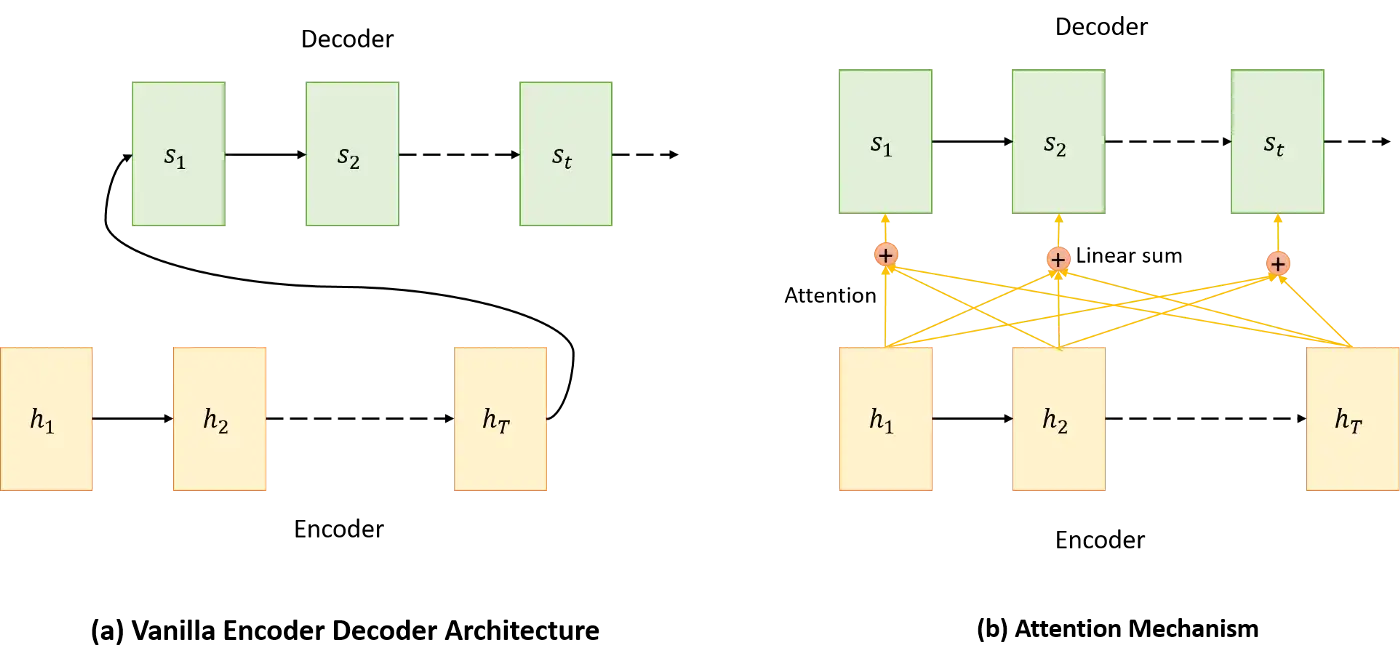
\includegraphics[width=\linewidth]{chapters/NLP/figures/attention.png}
    \caption{In vanilla encoder / decoder architectures, the decoder is only able to attend to the last hidden state of the encoder. Attention allows the decoder to attend to different parts of the input sequence in parallel.}
    \label{fig:attention}
\end{figure}
One way to address the vanishing gradient problem is to use a so called attention mechanisms.
The intuition behind them is to assign a weight to each part of the input sequence, indicating the importance of that part for the current task.
These weights are computed dynamically for each step in the processing of the input sequence and allow the model to focus on the most relevant parts of the sequence.

They are implemented as additional layers in the model that calculate the attention weights using a set of learnable parameters and use these weights to weight the hidden states of the RNN at each step in the processing of the input sequence.
The weighted hidden states are then combined and passed through a feedforward neural network to produce the final output.

There are several different types of attention mechanisms, including additive attention, multiplicative attention, and self-attention. Each of these mechanisms has its own strengths and weaknesses, and the choice of mechanism to use depends on the specific requirements of the task and the nature of the input data.

% The seminal paper introducing attention mechanisms is \cite{bahdanau2014neural},

\subsection{Transformers}
The development of attention mechanisms in RNNs laid the foundation for the development of the Transformer architecture, which is now the state-of-the-art in many natural language processing tasks.

The main drawback of attention mechanisms in RNNs is that they require sequential processing of the input sequence, which can be slow and inefficient for long sequences, and doesn't scale to large datasets.
The Transformer architecture was introduced as a solution, as it uses self-attention mechanisms to allow for parallel processing of the entire sequence.

\begin{figure}[h]
    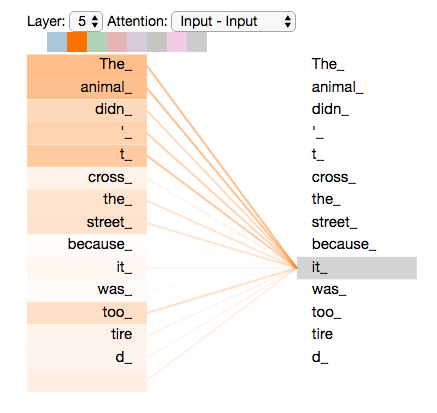
\includegraphics[width=\linewidth]{chapters/NLP/figures/self-attention.png}
    \caption{Here we visualize the attention weights for the word "it". The model learns to include the representation of "The Animal" as part of its encoding.}
    \label{fig:self-attention}
\end{figure}

Self-attention works by first embedding the input sequence into a continuous vector space. Then, for each position in the input sequence, the model calculates a set of attention scores, which indicate the degree of dependence between that position and all other positions in the sequence. These attention scores are used to compute a weighted sum of the input representations, which is then used as the input to the next layer of the model.
It is called self-attention because the model is able to put the representations of each token into context of all surrounding tokens (see Fig. \ref{fig:self-attention}).

\begin{figure}[h]
    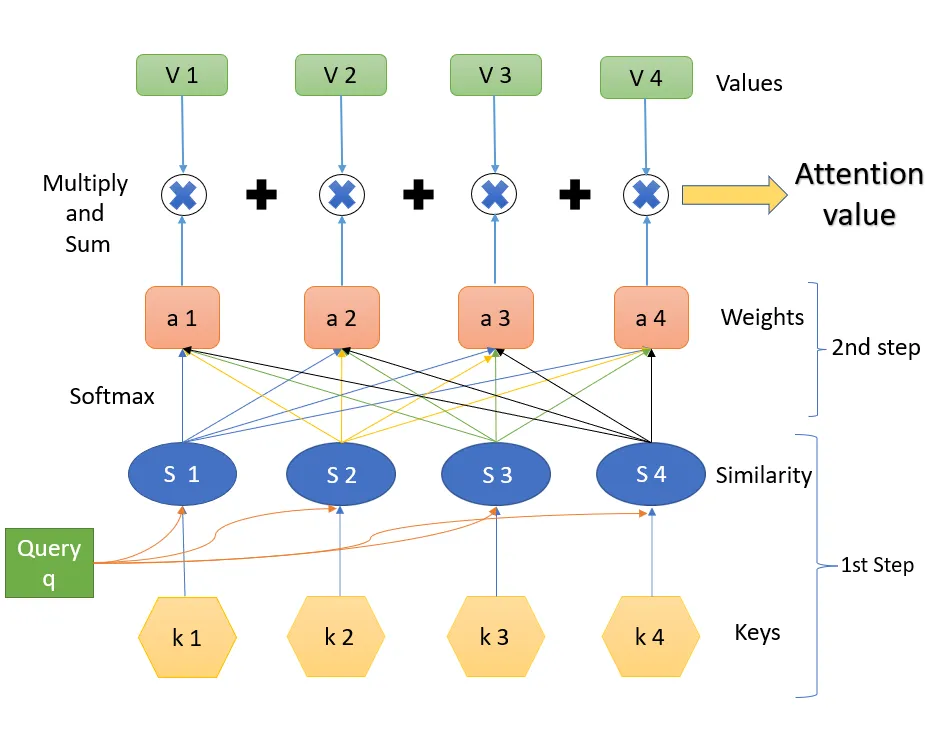
\includegraphics[width=\linewidth]{chapters/NLP/figures/queries_keys_values.png}
    \caption{Here we visualize the attention weights for the word "it". The model learns to include the representation of "The Animal" as part of its encoding.}
    \label{fig:queries-keys-values}
\end{figure}
Each token is assigned an embedding which is multiplied with three trainable weight matrices to obtain three vectors, called Queries, Keys, and Values.
The model first computes the dot product of the Query vector with each of the Key vectors, and then applies a softmax function to the resulting vector to obtain attention scores that are between 0 and 1 and sum to 1, where the softmax function is defined as:
\begin{equation}
    \text{softmax}(x_i) = \frac{e^{x_i}}{\sum_{j=1}^{n} e^{x_j}}
\end{equation}
Finally, the resulting vector of attention scores (Fig. \ref{fig:self-attention}) for each token is multiplied with the Value vectors to obtain the representation for this token (Fig. \ref{fig:queries-keys-values}).
The outputs of the self-attention mechanism are then passed through a feedforward neural network to produce the output of a so called \textit{encoder block}.
Many such encoder blocks are stacked on top of each other to form the encoder of the Transformer architecture.
In some architectures one wants to generate new text, for which we need a \textit{decoder}.
It has a very similar structure, but we will defer that discussion here.
For more details on the Transformer architecture, we refer the reader to \cite{vaswani2017attention} and for a more intuitive explanation we recommend \cite{illustratedtransformer}.

\subsubsection{Pre-training and Finetuning}
The state of the art in NLP is currently dominated by Transformer-based models, which are trained using a two-stage process called \textit{pre-training} and \textit{fine-tuning}. Starting with a model pre-trained on a broad set of topics significantly reduces the amount of task specific training data required to achieve great performance.

Pre-training refers to the process of training a model on a large corpus\footnote{BooksCorpus (800M words, Wikipedia 2,500M words)}\cite{bertpaper} of text, sometimes in multiple languages, or on domain-specific datasets\footnote{\texttt{BioBERT\cite{DBLP:journals/corr/abs-1901-08746}}}\footnote{\texttt{Bio\textunderscore ClinicalBERT\cite{clinicalbert}}}, but without any task-specific supervision.
The model is trained to predict masked tokens in a sequence, or to reconstruct the input sequence itself, using only the context information provided by surrounding tokens.
This process enables the model to learn general language patterns and relationships between words and concepts, and can be compared to a human learning a new language.
Just as a human needs to understand the basic rules and patterns of a language before they can use it to apply it effectively, a model needs to do the same.
Pre-trained Transformer models are freely available for download\footnote{Huggingface} and can be used as a starting point for many NLP tasks.
They are able to produce robust sentence embeddings with a fine grained understanding of syntactic structure, semantics, and general knowledge of the world.
You can also pre-train your own model from scratch, but this requires a lot of data, time and money, and is rarely worth the investment.

Fine-tuning on the other hand refers to the process of adapting the pre-trained model on a much smaller dataset to a specific task, such as classification, sentiment analysis, question answering, or machine translation.
This can be compared to a human adapting their language skills to a specific context.
For example, a person who has learned a new language may need to modify their language skills to fit a particular situation, such as a formal business setting or a casual conversation with friends.
During fine-tuning, a task-specific layer is added on the on top of the pre-trained model and either only that layer or the entire network is trained end-to-end on the task-specific data.

\subsection{Practical Considerations}
In contemporary architectures there are millions to hundreds of billions of parameters, and updating them efficiently is crucial.

\subsubsection{Feeding Data to the Model}
\begin{figure}[h]
    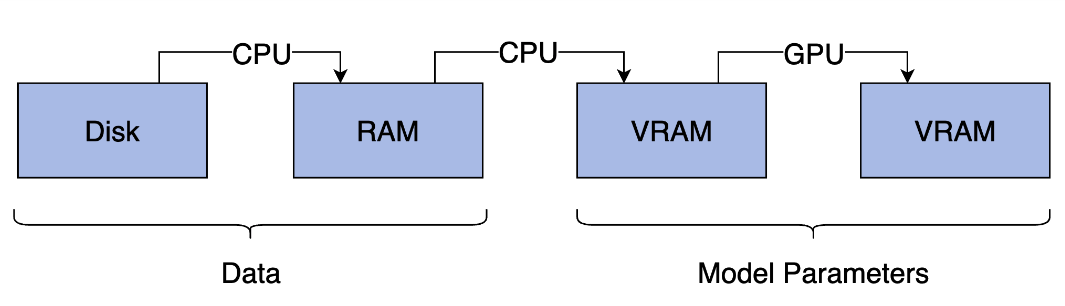
\includegraphics[width=\linewidth]{chapters/NLP/figures/ram_cpu_vram.png}
    \caption{Data needs to be moved from disk to RAM to VRAM so that it can be used to update the model parameters.}
    \label{fig:ram_cpu_vram}
\end{figure}
Model parameters are stored in GPU memory (known as VRAM); in order to update them, the GPU needs to process data from the training set.
After downloading the data from cloud storage it resides on local disk, from where it needs to be moved to RAM and finally VRAM.
Loading data into the model needs to be fast, or we run the risk of starving the GPU, meaning the GPU processes each batch of data faster than the CPU can deliver the next one, leading to low resource utilization and slow training.
We use PyTorch's \pythoninline{DataLoader} class to parallelize this process across multiple CPU workers.
A \pythoninline{DataLoader} takes as argument a \pythoninline{Dataset} and provides a stream of batches of data.
The \textit{batch size} is an important parameter that needs to be tuned on a case by case basis, as we will explain in the next section.


\subsubsection{Mini-batch Gradient Descent}
To optimize the parameters as outlined in Eq. \ref{eq:optimization} we need to evaluate the gradient of the loss function given the data $(x_i, y_i)$.
To compute the optimial update step we need to sum over all samples in the dataset, compute and store all the gradients, update the parameters once, and repeat the process until convergence.
This, however is not practical, given the size of typical datasets and the number of model parameters -- each step would be very computationally expensive and the training slow.

On the other end of the spectrum we could use only a single sample to compute approximations of the optimal gradients, and they will take us close to the global minimum.
This method is called \textit{stochastic gradient descent} and generally works well, but it comes with some tradeoffs:
\begin{itemize}
    \item Loading single samples from the dataset is slow, due to CPU, RAM and bus overhead when copying data to VRAM
    \item There is overhead in the GPU related to scheduling of compute operations
    \item The gradients are much more noisy than the optimal ones, and the model will learn more slowly (see Fig. \ref{fig:mini-batch})
\end{itemize}
There is a happy middle ground called \textit{mini-batch gradient descent} which is a combination of stochastic gradient descent with mini-batches.
Using mini-batches allows for a more accurate estimate of the gradient, and reduces the overhead per sample, as we can take advantage of hardware accelerated vectorized compute operations in CPUs and GPUs.
In practice, we will choose a batch size that is much smaller than the number of samples in the dataset, and as big as possible without running out of VRAM, where the latter condition is typically the more relevant constraint.

\begin{figure}[h]
    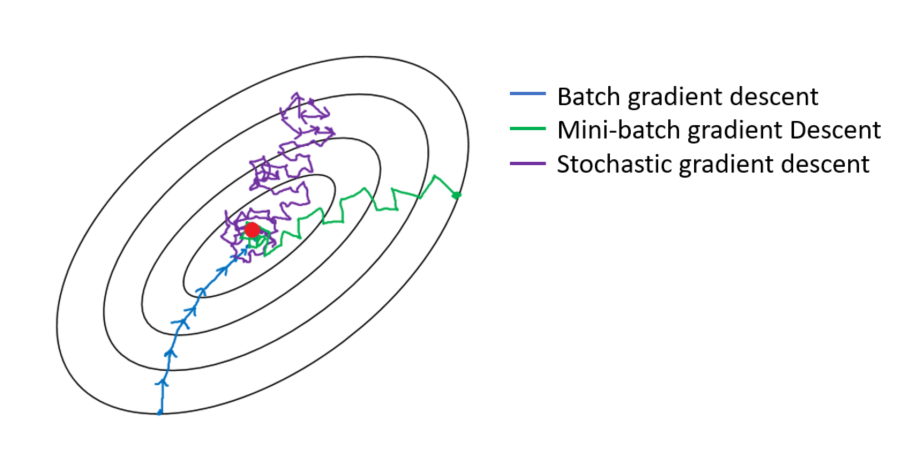
\includegraphics[width=\linewidth]{chapters/NLP/figures/mini-batch.png}
    \caption{Batch vs mini-batch vs stochastic gradient descent}
    \label{fig:mini-batch}
\end{figure}

Many optimization algorithms exist that aim to minimize the objective loss function that represents a deep learning model. Stochastic
gradient descent is often a good first choice for this optimization. It requires tuning the \textit{learning rate} parameter, which controls how much the parameters
will adjust on each step of the iteration after calculating the relative error of the model with respect to each of these parameters. A large learning rate
will often get stuck in local optima because it is unable to find the minimum in a complex multi-dimensional optimization space, whereas a smaller learning rate
might take too long to train. Learning rate schedules are often used that aim to get the best of both worlds. One schedule that is often used is to
begin with a higher learning rate and to slowly decay it as you train. This often allows for faster overall training but still converging to a lower final loss. 
Another technique that is used in practice is also to cycle learning rates between high and low numbers, as this allows the loss functions to escape
from local optima and finely explore other parts of the decision space.

As mentioned, mini-batch gradient descent is not the only loss function available to us. Most deep learning libraries support many others that
automatically compute these partial derivatives for each parameter and adjust them on every backpropagation pass. Some incorporate weighted averages to establish
a momentum term to smooth out the jumpiness of the loss value. Others have learning rates that exist for each separate parameter and not a single global learning rate.
The Adam optimizer is a good first choice that combines these techniques and works out of the box quite well for a variety of NLP problems.


\subsubsection{Regularization}
\begin{figure}[h]
    \centering
    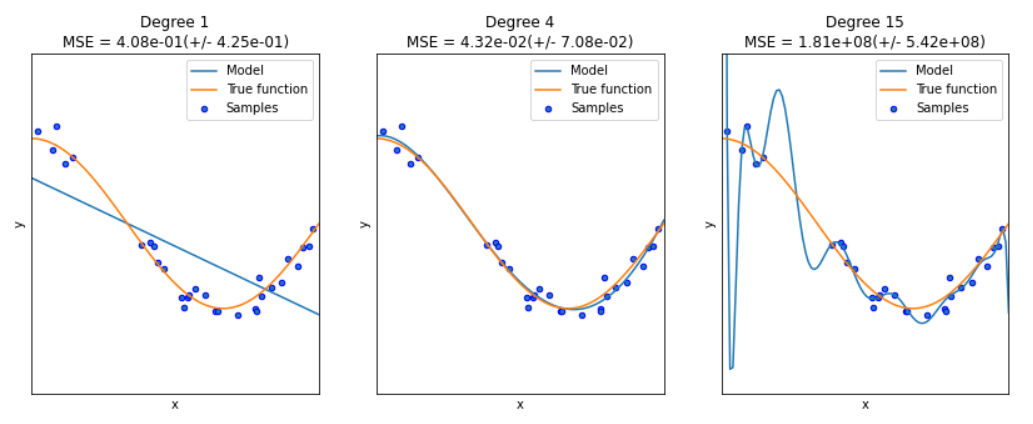
\includegraphics[width=1.2\textwidth]{chapters/NLP/figures/over_and_underfitting.png}
    \caption{Left: Underfitting, a straight line doesn't fit  the data well.
    Right: Overfitting, a complex curve fits the (training) data perfectly, but will likely not generalize well.
    Center: The model and true underlying function match closely.}
    \label{fig:over_and_underfitting}
\end{figure}
A common problem in ML is the balance between over- and underfitting (Figure \ref{fig:over_and_underfitting}).
Underfitting can happen when the model is too simple, i.e. it is not able to capture the underlying function (rarely a problem in deep learning).
Overfitting happens when the model is too complex or has too many degrees of freedom, such that it can fit the training data well, but does not capture the essence of the true data generating process, leading to poor generalization performance when applied to new data.

An easy way to detect these issues is by observing training and validation metrics as a function training steps or epochs, called learning curves.
We want to see that both, training and validation metrics continue to improve as training progresses until they both taper off at a certain point.
Note that it is normal to see a difference in the absolute value and rate of change between the training and validation metrics.
This is called the generalization error, and is nothing to be too concerned about, ultimately only the validation and test metrics are relevant.
What \textit{is} problematic is if we observe that the validation metrics start to get worse, while the training metrics continue to improve -- this is a clear sign of overfitting and we should stop the training early (Figure \ref{fig:learning_curves}).
\begin{figure}
    \centering
    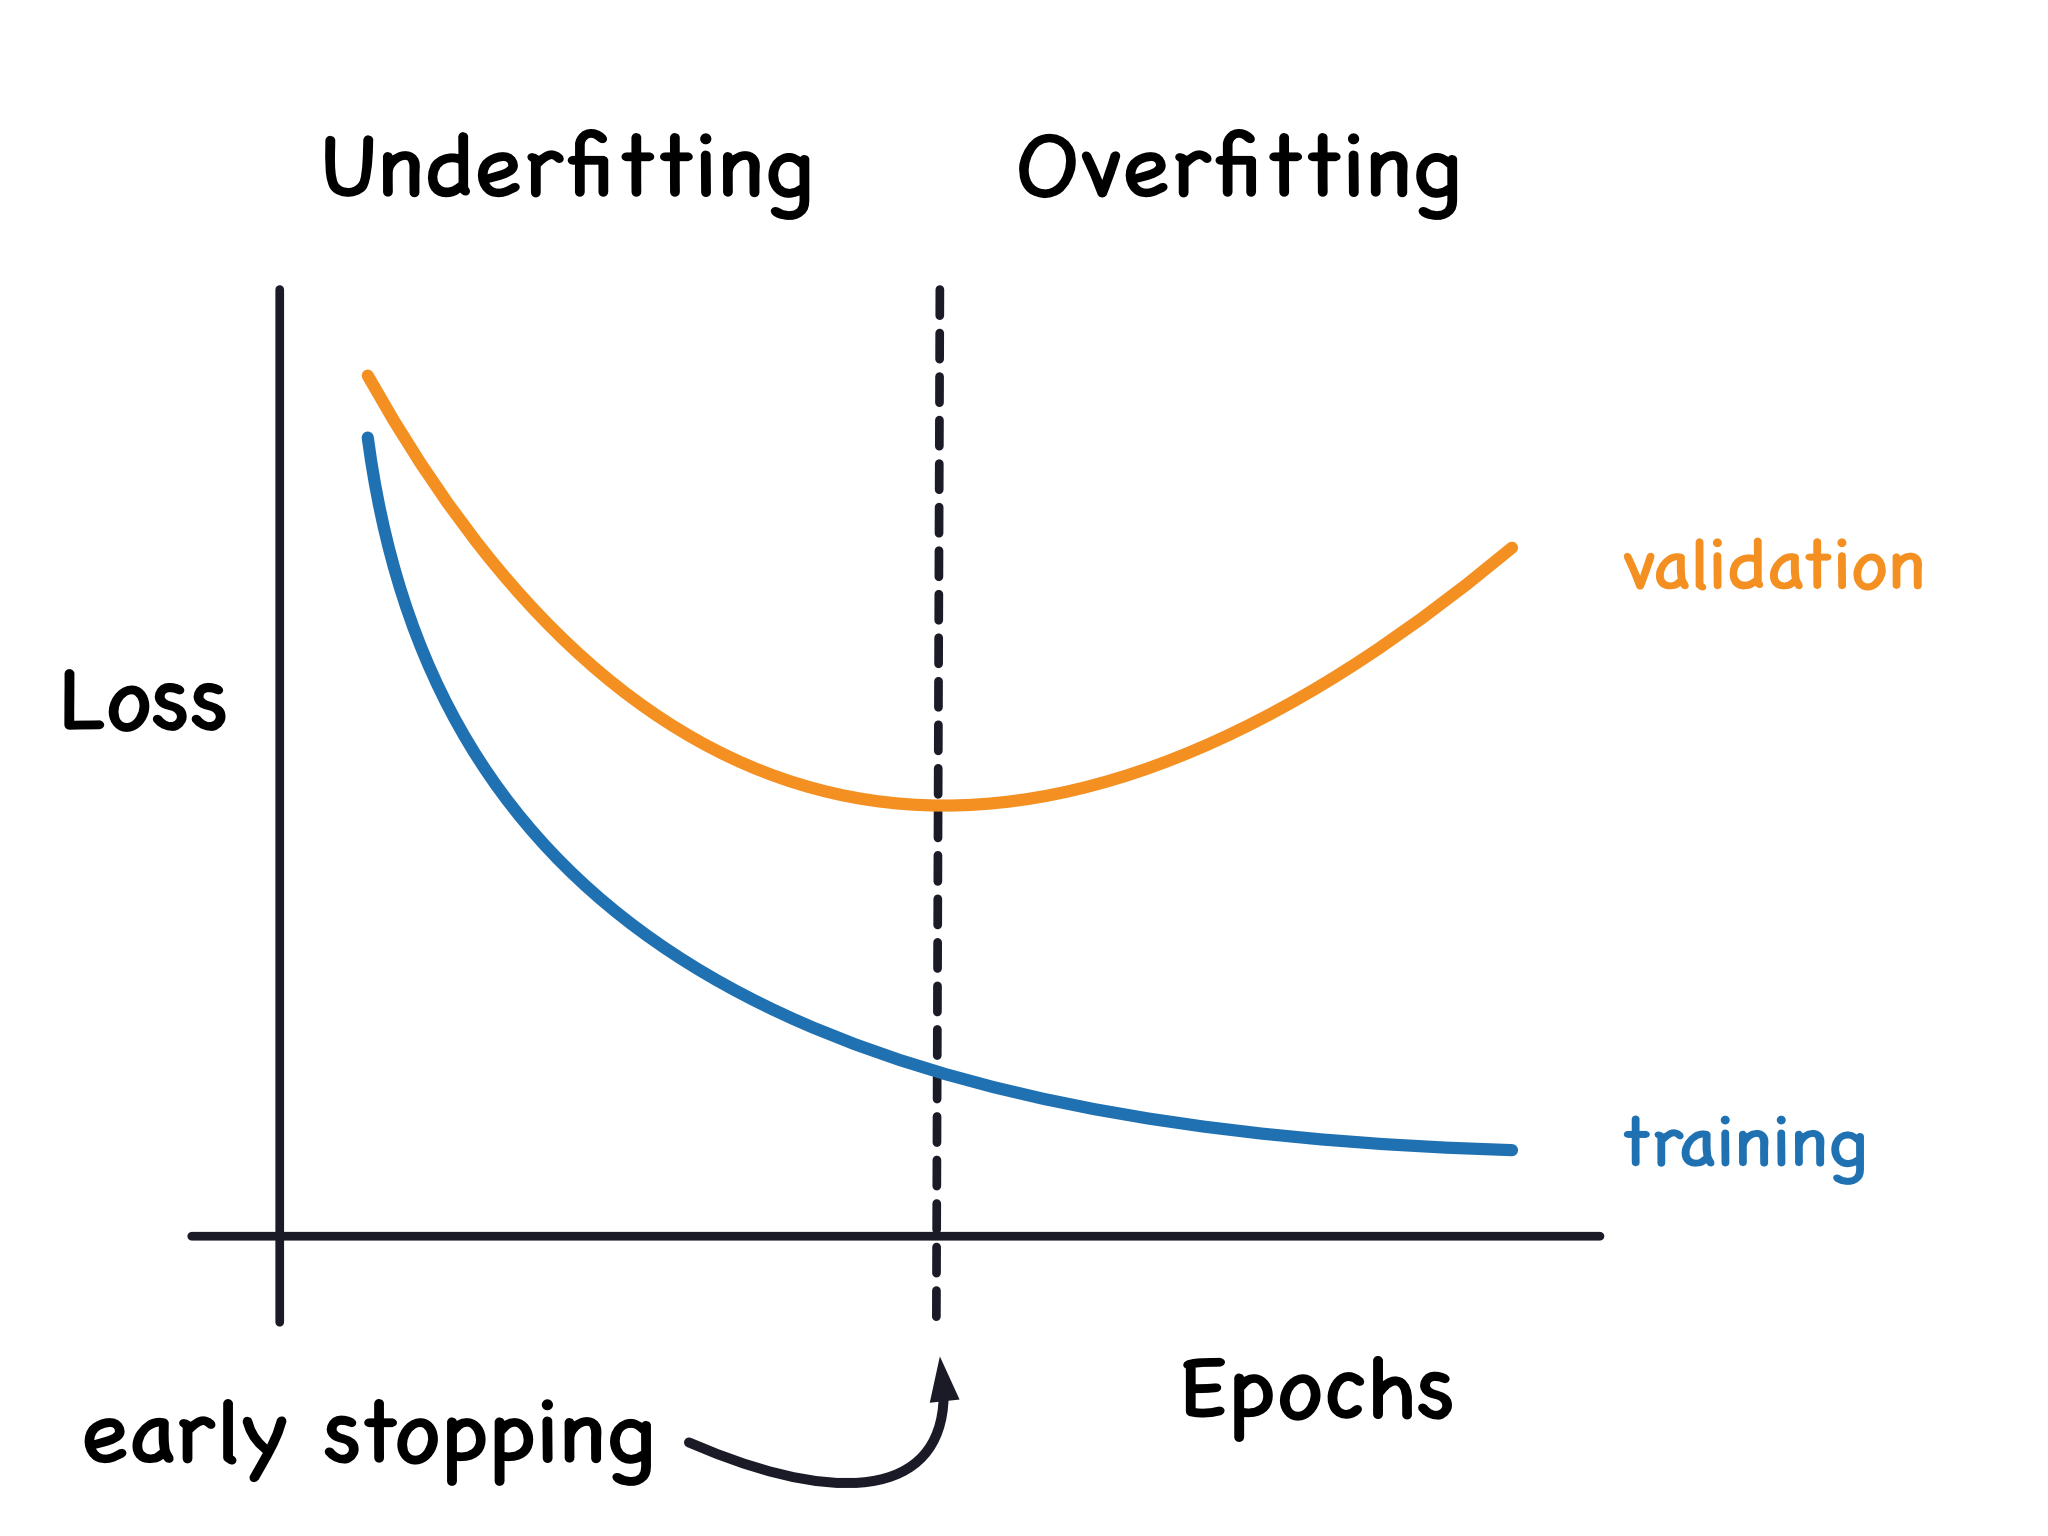
\includegraphics[width=0.8\textwidth]{chapters/NLP/figures/learning_curves.png}
    \caption{Learning curves, the training and validation loss are plotted as a function of the number of training steps / epochs.}
    \label{fig:learning_curves}
\end{figure}
To address underfitting, the easiest remedy is to increase the complexity of the model (e.g. add more layers) or to increase the number of training steps.
We can also try to add more features to the dataset, such as adding more words to the vocabulary.
When dealing with overfitting in deep learning, we usually don't want to reduce the model complexity, but instead add \textit{regularization} and more data.
Regularization is a technique that restricts the freedom of the model, for example by introducing a penalty on the magnitude of the model parameters.
For this, the loss functions in Table \ref{table:losses} are modified as
\begin{equation}
    \tilde{L}(\theta) = L(\theta) + \frac{1}{2} \sum_{i} |\theta_i|^2.
\end{equation}

Another common technique is to add \textit{dropout}, where a fraction of neurons is randomly turned off for each training step.
This ensures that each neuron has a unique purpose and learns to detect a specific set of features in the data, without co-adapting to the output of other neurons.
Another interpretation of dropout is that it can be seen as an approximation to a bagging technique, where the outputs of different models at each iteration are averaged, leading to an overall reduction in errors if they are uncorrelated.
This tends to reduce generalization error, prevent the model from fitting to irrelevant details, and make it more robust to noise.

There are many other regularization techniques that are used in practice. They are all designed to reduce
generalization error, and not training error. Often they come in the flavor of the additional terms added to the
objective function, as exemplified in Equation 2.3, or as model restrictions, such as dropout. Another common technique
is on the dataset level, wherein practitioners will directly augment datasets. You will see this happen often in image classification
tasks where a dataset will create random copies of samples that are rotated and stretched in different directions to make
the model robust to such invariance. Direct injection of noise, randomly-generated numbers, also occurs on both the input
as well as label side. 
